\section{Allievi}
\subsection{Panoramica allievi}
\begin{figure}[H]
\centering
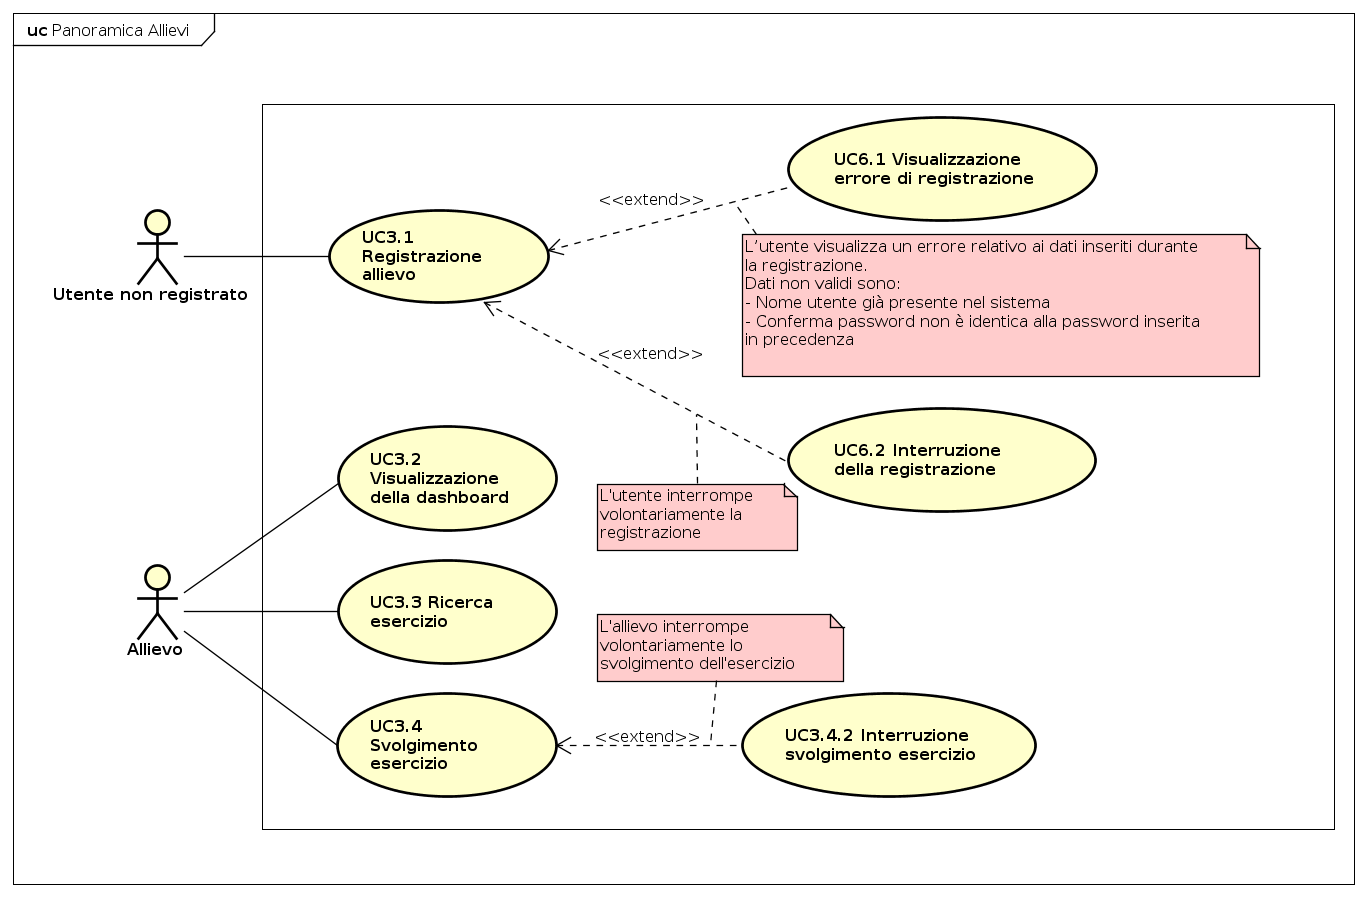
\includegraphics[width=17cm]{img/Panoramica Allievi.png} 
\caption{Panoramica allievi}\label{fig:31}
\end{figure}

\subsection{UC 3.1 - Registrazione allievo}
\begin{figure}[H]
\centering
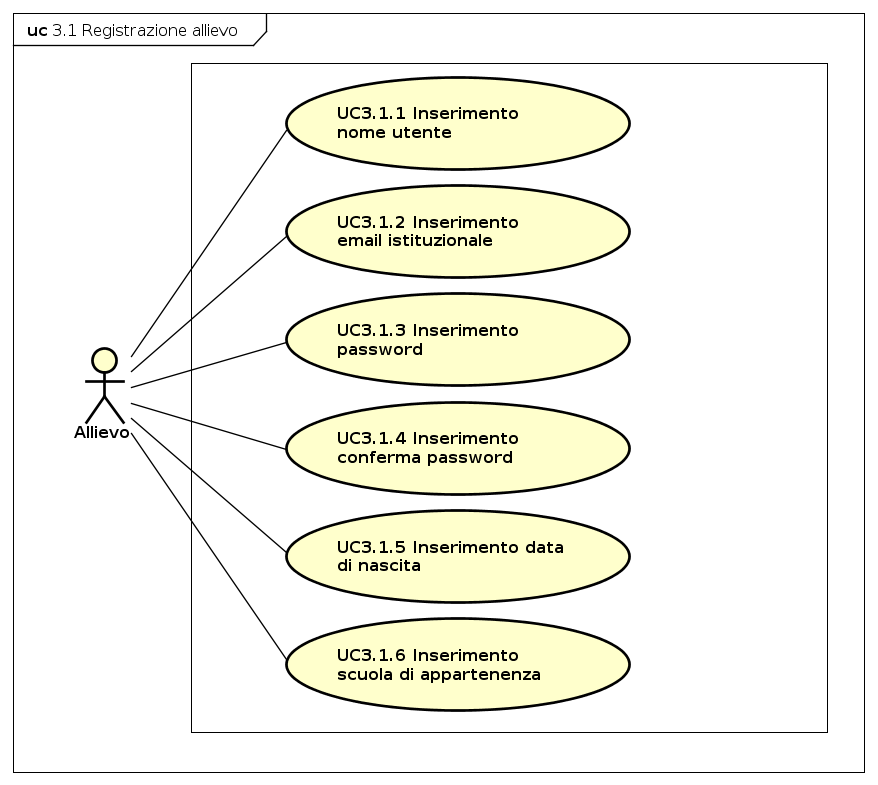
\includegraphics[width=17cm]{img/UC31.png} 
\caption{Caso d'uso 3.1}\label{fig:31}
\end{figure}
\begin{itemize}
\item[•]\textbf{Attori}: Utente non registrato;
\item[•]\textbf{Descrizione}: L’utente non registrato compila il form di registrazione relativo all’allievo completando la registrazione;
\item[•]\textbf{Precondizione}: L’utente non è registrato;
\item[•]\textbf{Postcondizione}: L’utente si è registrato come allievo;
\item[•]\textbf{Flusso degli eventi principale}:
\begin{enumerate}
\item UC 3.1.1 - Inserimento nome utente;
\item UC 3.1.2 - Inserimento email istituzionale;
\item UC 3.1.3 - Inserimento password;
\item UC 3.1.4 - Inserimento conferma password;
\item UC 3.1.5 - Inserimento data di nascita;
\item UC 3.1.6 - Inserimento scuola di appartenenza.
\end{enumerate}
\item[•]\textbf{Estensioni}:
\begin{enumerate}
\item UC 6.1 - Visualizzazione errore di registrazione;
\item UC 6.2 - Interruzione della registrazione.
\end{enumerate}
\end{itemize}

\subsubsection{UC 3.1.1 - Inserimento nome utente}
\begin{itemize}
\item[•]\textbf{Attori}: Utente non registrato;
\item[•]\textbf{Descrizione}: L’utente inserisce un nome utente durante la registrazione;
\item[•]\textbf{Precondizione}: L’utente non è registrato;
\item[•]\textbf{Postcondizione}: L’utente ha inserito un nome utente;
\end{itemize}

\subsubsection{UC 3.1.2 - Inserimento email istituzionale}
\begin{itemize}
\item[•]\textbf{Attori}: Utente non registrato;
\item[•]\textbf{Descrizione}: L’utente inserisce la sua email istituzionale durante la registrazione;
\item[•]\textbf{Precondizione}: L’utente non è registrato;
\item[•]\textbf{Postcondizione}: L’utente ha inserito una email istituzionale;
\end{itemize}

\subsubsection{UC 3.1.3 - Inserimento password}
\begin{itemize}
\item[•]\textbf{Attori}: Utente non registrato;
\item[•]\textbf{Descrizione}: L’utente inserisce una password durante la registrazione;
\item[•]\textbf{Precondizione}: L’utente non è registrato;
\item[•]\textbf{Postcondizione}: L’utente ha inserito una password;
\end{itemize}

\subsubsection{UC 3.1.4 - Inserimento conferma password}
\begin{itemize}
\item[•]\textbf{Attori}: Utente non registrato;
\item[•]\textbf{Descrizione}: L’utente inserisce la conferma della password durante la registrazione;
\item[•]\textbf{Precondizione}: L’utente non è registrato;
\item[•]\textbf{Postcondizione}: L’utente ha inserito la conferma della password;
\end{itemize}

\subsubsection{UC 3.1.5 - Inserimento data di nascita}
\begin{itemize}
\item[•]\textbf{Attori}: Utente non registrato;
\item[•]\textbf{Descrizione}: L’utente inserisce la sua data di nascita durante la registrazione;
\item[•]\textbf{Precondizione}: L’utente non è registrato;
\item[•]\textbf{Postcondizione}: L’utente ha inserito la sua data di nascita;
\end{itemize}

\subsubsection{UC 3.1.6 - Inserimento scuola di appartenenza}
\begin{itemize}
\item[•]\textbf{Attori}: Utente non registrato;
\item[•]\textbf{Descrizione}: L’utente inserisce la sua scuola di appartenenza durante la registrazione;
\item[•]\textbf{Precondizione}: L’utente non è registrato;
\item[•]\textbf{Postcondizione}: L’utente ha inserito la sua scuola di appartenenza;
\end{itemize}

\subsection{UC 3.2 - Visualizzazione della dashboard\ped{G}}
\begin{figure}[H]
\centering
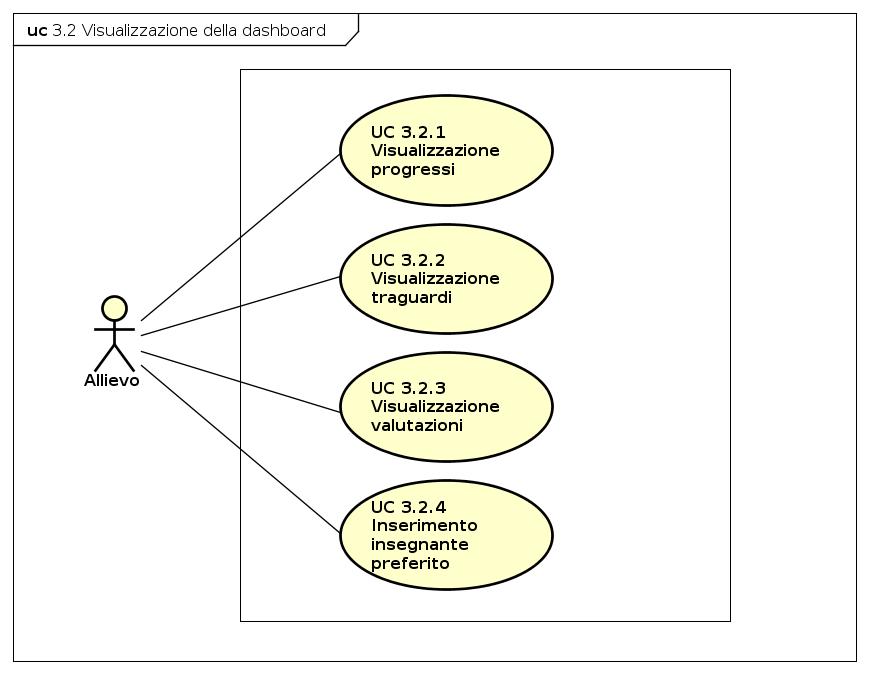
\includegraphics[width=17cm]{img/UC32.png} 
\caption{Caso d'uso 3.2}\label{fig:32}
\end{figure}
\begin{itemize}
\item[•]\textbf{Attori}: Allievo;
\item[•]\textbf{Descrizione}: L’allievo apre la propria dashboard\ped{G};
\item[•]\textbf{Precondizione}: Il sistema offre la possibilità di visualizzare la propria dashboard\ped{G};
\item[•]\textbf{Postcondizione}: L’allievo ha aperto la dashboard\ped{G} e può vederne tutte le componenti;
\item[•]\textbf{Flusso degli eventi principale}:
\begin{enumerate}
\item UC 3.2.1 - Visualizzazione progressi;
\item UC 3.2.2 - Visualizzazione traguardi;
\item UC 3.2.3 - Visualizzazione valutazioni;
\item UC 3.2.4 - Inserimento insegnante preferito.
\end{enumerate}
\end{itemize}

\subsubsection{UC 3.2.1 - Visualizzazione progressi}
\begin{itemize}
\item[•]\textbf{Attori}: Allievo;
\item[•]\textbf{Descrizione}: L’allievo visualizza i suoi progressi: numero di esercizi svolti, corretti ed errati;
\item[•]\textbf{Precondizione}: Il sistema offre la possibilità di visualizzare i progressi raggiunti;
\item[•]\textbf{Postcondizione}: L’allievo può visualizzare i propri progressi;
\end{itemize}

\subsubsection{UC 3.2.2 - Visualizzazione traguardi}
\begin{itemize}
\item[•]\textbf{Attori}: Allievo;
\item[•]\textbf{Descrizione}: L’allievo visualizza i traguardi raggiunti;
\item[•]\textbf{Precondizione}: Il sistema offre la possibilità di visualizzare i traguardi;
\item[•]\textbf{Postcondizione}: L’allievo può visualizzare tutti i traguardi raggiunti;
\end{itemize}

\subsubsection{UC 3.2.3 - Visualizzazione valutazioni}
\begin{itemize}
\item[•]\textbf{Attori}: Allievo;
\item[•]\textbf{Descrizione}: L’allievo visualizza le valutazioni di tutti gli esercizi svolti, sia esercizi assegnati che svolti indipendentemente;
\item[•]\textbf{Precondizione}: Il sistema offre la possibilità di visualizzare le valutazioni;
\item[•]\textbf{Postcondizione}: L’allievo può visualizzare tutte le valutazioni ricevute;
\end{itemize}

\subsubsection{UC 3.2.4 - Inserimento insegnante preferito}
\begin{itemize}
\item[•]\textbf{Attori}: Allievo;
\item[•]\textbf{Descrizione}: L’allievo inserisce il nome utente dell’insegnante da prediligere quando riceve la correzione di un esercizio. L’inserimento di un nuovo insegnante sovrascrive il precedente;
\item[•]\textbf{Precondizione}: Il sistema offre la possibilità di inserire un insegnante preferito;
\item[•]\textbf{Postcondizione}: L’allievo ha inserito un insegnante preferito;
\end{itemize}

\subsection{UC 3.3 - Ricerca esercizio}
\begin{figure}[H]
\centering
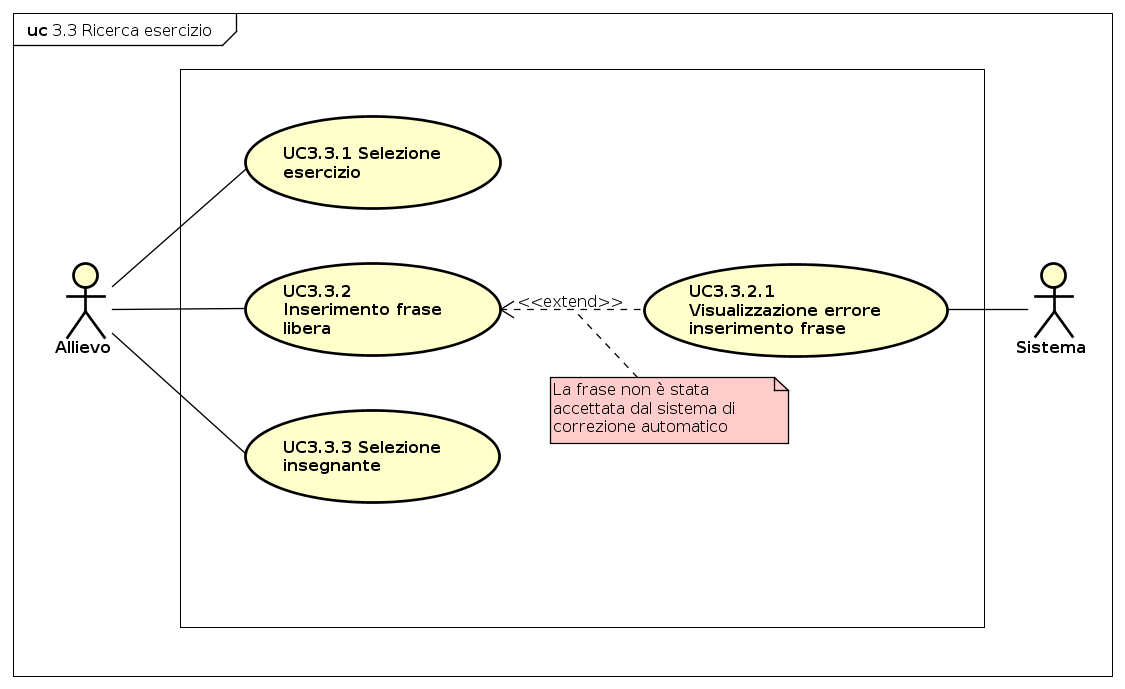
\includegraphics[width=17cm]{img/UC33.png} 
\caption{Caso d'uso 3.3}\label{fig:33}
\end{figure}
\begin{itemize}
\item[•]\textbf{Attori}: Allievo;
\item[•]\textbf{Descrizione}: L’allievo ricerca un esercizio attraverso frasi suggerite dal sistema o attraverso l’inserimento di una frase libera;
\item[•]\textbf{Precondizione}: Il sistema offre la possibilità di ricercare un esercizio;
\item[•]\textbf{Postcondizione}: L’allievo può navigare una lista di esercizi consigliati o inserire una frase;
\item[•]\textbf{Flusso degli eventi principale}:
\begin{enumerate}
\item UC 3.3.1 - Selezione esercizio;
\item UC 3.3.2 - Inserimento frase libera.
\end{enumerate}
\end{itemize}

\subsubsection{UC 3.3.1 - Selezione esercizio}
\begin{itemize}
\item[•]\textbf{Attori}: Allievo;
\item[•]\textbf{Descrizione}: L’allievo seleziona un esercizio nella lista delle frasi consigliate;
\item[•]\textbf{Precondizione}: Il sistema offre la possibilità di visualizzare una lista di esercizi;
\item[•]\textbf{Postcondizione}: Un esercizio è stato correttamente selezionato;
\item[•]\textbf{Flusso degli eventi principale}:
\begin{enumerate}
\item UC 3.3.1.1 - Selezione insegnante;
\item UC 3.4 - Svolgimento esercizio.
\end{enumerate}
\end{itemize}

\subsubsection{UC 3.3.1.1 - Selezione insegnante}\begin{figure}[H]
\centering
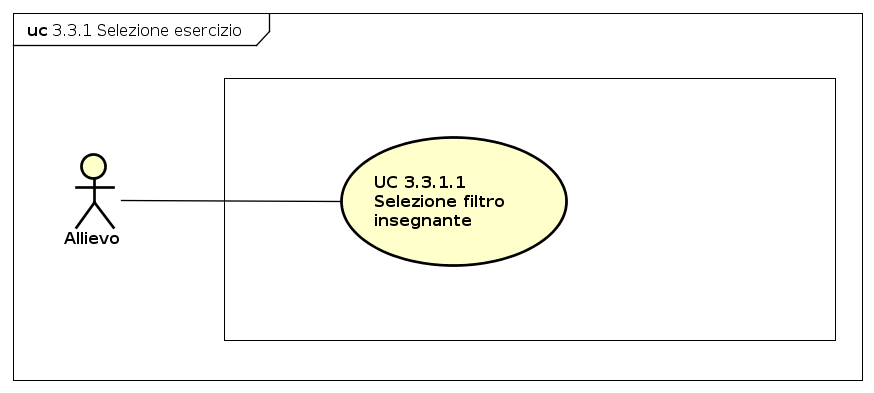
\includegraphics[width=17cm]{img/UC331.png} 
\caption{Caso d'uso 3.3.1}\label{fig:331}
\end{figure}
\begin{itemize}
\item[•]\textbf{Attori}: Allievo;
\item[•]\textbf{Descrizione}: L’allievo seleziona l’insegnante da cui vuole ricevere la correzione dell’esercizio, se nessun insegnante ha predisposto quella frase verrà utilizzato il sistema di correzione automatico. Quando è possibile l’insegnante preferito viene selezionato automaticamente;
\item[•]\textbf{Precondizione}: L’allievo ha selezionato un esercizio;
\item[•]\textbf{Postcondizione}: L’allievo ha selezionato da chi vuole ricevere la correzione;
\end{itemize}

\subsubsection{UC 3.3.2 - Inserimento frase libera}
\begin{itemize}
\item[•]\textbf{Attori}: Allievo;
\item[•]\textbf{Descrizione}: L’allievo inserisce la propria frase in modo da ricevere l’analisi grammaticale di essa;
\item[•]\textbf{Precondizione}: Il sistema offre la possibilità di inserire una frase;
\item[•]\textbf{Postcondizione}: Una frase è stata correttamente inserita;
\item[•]\textbf{Flusso degli eventi principale}:
\begin{enumerate}
\item UC 3.4.3 - Visualizzazione soluzione.
\end{enumerate}
\item[•]\textbf{Estensioni}:
\begin{enumerate}
\item UC 3.3.2.1 - Visualizzazione errore inserimento frase.
\end{enumerate}
\end{itemize}

\subsubsection{UC 3.3.2.1 - Visualizzazione errore inserimento frase}
\begin{itemize}
\item[•]\textbf{Attori}: Allievo, Libreria di pos-tagging;
\item[•]\textbf{Descrizione}: La frase inserita non è accettata dalla libreria di pos-tagging. L'allievo visualizza un errore e può inserire una nuova frase;
\item[•]\textbf{Precondizione}: L’allievo ha provato ad inserire una frase;
\item[•]\textbf{Postcondizione}: L’allievo ha visualizzato il messaggio di errore e può inserire una nuova frase;
\end{itemize}

\subsection{UC 3.4 - Svolgimento esercizio}
\begin{figure}[H]
\centering
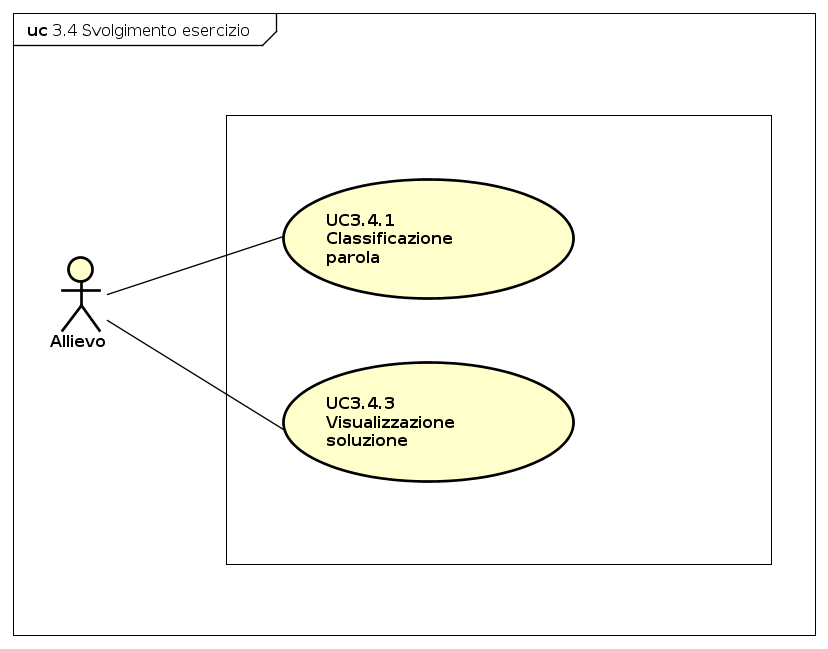
\includegraphics[width=17cm]{img/UC34.png} 
\caption{Caso d'uso 3.4}\label{fig:34}
\end{figure}
\begin{itemize}
\item[•]\textbf{Attori}: Allievo;
\item[•]\textbf{Descrizione}: L’allievo può svolgere l’esercizio scegliendo le classi grammaticali per ciascuna parola da una apposita lista;
\item[•]\textbf{Precondizione}: L’allievo ha selezionato un esercizio;
\item[•]\textbf{Postcondizione}: L’allievo ha svolto un esercizio;
\item[•]\textbf{Flusso degli eventi principale}:
\begin{enumerate}
\item UC 3.4.1 - Classificazione parola;
\item UC 3.4.3 - Visualizzazione soluzione.
\end{enumerate}
\item[•]\textbf{Estensioni}:
\begin{enumerate}
\item UC 3.4.2 - Interruzione svolgimento esercizio.
\end{enumerate}
\end{itemize}

\subsubsection{UC 3.4.1 - Classificazione parola}
\begin{itemize}
\item[•]\textbf{Attori}: Allievo;
\item[•]\textbf{Descrizione}: L’allievo seleziona la classe grammaticale di una parola da una lista predefinita;
\item[•]\textbf{Precondizione}: Il sistema dà la possibilità di selezionare la classe grammaticale di una parola;
\item[•]\textbf{Postcondizione}: L’allievo ha selezionato la classe grammaticale di una parola;
\end{itemize}

\subsubsection{UC 3.4.2 - Interruzione svolgimento esercizio}
\begin{itemize}
\item[•]\textbf{Attori}: Allievo;
\item[•]\textbf{Descrizione}: L’allievo interrompe l’esercizio, scartando i dati inseriti fino a quel momento, e ritorna nella sezione di ricerca di un esercizio;
\item[•]\textbf{Precondizione}: L’allievo ha iniziato a svolgere un esercizio;
\item[•]\textbf{Postcondizione}: L’allievo ha interrotto l’esercizio, torna nella sezione di ricerca di un esercizio;
\end{itemize}

\subsubsection{UC 3.4.3 - Visualizzazione soluzione}
\begin{itemize}
\item[•]\textbf{Attori}: Allievo, Libreria di pos-tagging;
\item[•]\textbf{Descrizione}: L’allievo visualizza la correzione secondo l’insegnante selezionato in precedenza. Se era stata inserita una frase libera la correzione viene eseguita dal sistema di correzione automatico;
\item[•]\textbf{Precondizione}: L’allievo ha svolto un esercizio oppure ha inserito una frase libera;
\item[•]\textbf{Postcondizione}: L’allievo ha visualizzato la soluzione dell’esercizio;
\item[•]\textbf{Flusso degli eventi principale}:
\begin{enumerate}
\item UC 3.4.3.1 - Selezione soluzione alternativa.
\end{enumerate}
\end{itemize}

\subsubsection{UC 3.4.3.1 - Selezione soluzione alternativa}
\begin{figure}[H]
\centering
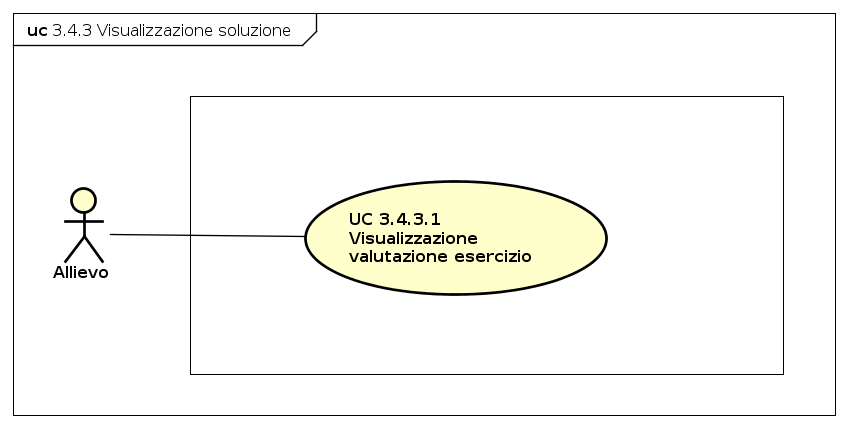
\includegraphics[width=17cm]{img/UC343.png} 
\caption{Caso d'uso 3.4.3}\label{fig:343}
\end{figure}
\begin{itemize}
\item[•]\textbf{Attori}: Allievo;
\item[•]\textbf{Descrizione}: L’allievo può selezionare da una lista una soluzione alternativa proposta dallo stesso insegnante;
\item[•]\textbf{Precondizione}: L’allievo ha visualizzato la correzione dell’esercizio svolto;
\item[•]\textbf{Postcondizione}: L’allievo ha visualizzato una soluzione alternativa dell’esercizio svolto;
\end{itemize}

\section{Estensioni registrazione}
\subsection{UC 6.1 - Visualizzazione errore di registrazione}
\begin{itemize}
\item[•]\textbf{Attori}: Utente non registrato;
\item[•]\textbf{Descrizione}: L’utente visualizza un errore relativo ai dati inseriti durante la registrazione.
Dati non validi sono:
 - Nome utente già presente nel sistema
 - Conferma password non è identica alla password inserita in precedenza;
\item[•]\textbf{Precondizione}: L’utente ha cominciato la registrazione;
\item[•]\textbf{Postcondizione}: La registrazione non viene effettuata, viene visualizzato un messaggio relativo ai dati compilati in modo errato;
\end{itemize}

\subsection{UC 6.2 - Interruzione della registrazione}
\begin{itemize}
\item[•]\textbf{Attori}: Utente non registrato;
\item[•]\textbf{Descrizione}: L’utente interrompe volontariamente la registrazione;
\item[•]\textbf{Precondizione}: L’utente ha cominciato la registrazione;
\item[•]\textbf{Postcondizione}: La registrazione non viene effettuata;
\end{itemize}
